
\section{Mouselab MDP}
\label{sec:mouselab_mdp}

% Shortened version of RLDM paper introducing mouselab-MDP
%\fl{TODO: Fred and Falk, Paul and Sayan can help too}
Planning, like all of cognition, is a mental process that cannot be observed directly. Thus, to compare people's planning strategy to the bounded-optimal planning strategy, we first had to make it observable. To do so, we developed a process tracing paradigm for the study of planning \cite{CallawayLiederKrueger2017}. Our Mouselab-MDP paradigm is inspired by the Mouselab paradigm \citep{Payne1993} that traces how people choose between multiple risky gambles. The basic idea is to externalize people's mental simulations of alternative action sequences. To do so, the Mouselab-MDP paradigm presents participants with a route planning problem where each move earns or loses an initially unknown amount of money. The participant's goal is to choose a route in such a way that they earn as much money as possible. To find out how much money a transition would yield the participant has to click on it and pay a fee. Each click is recorded and the recorded sequence of clicks reveals which paths participants mentally simulated and in which order. This is because finding out the payoff for a simulated move requires clicking on it. Figure \ref{fig:MouselabMDP} illustrates the Mouselab-MDP paradigm with the task used to teach people how to plan better.

\begin{figure}
    \centering
    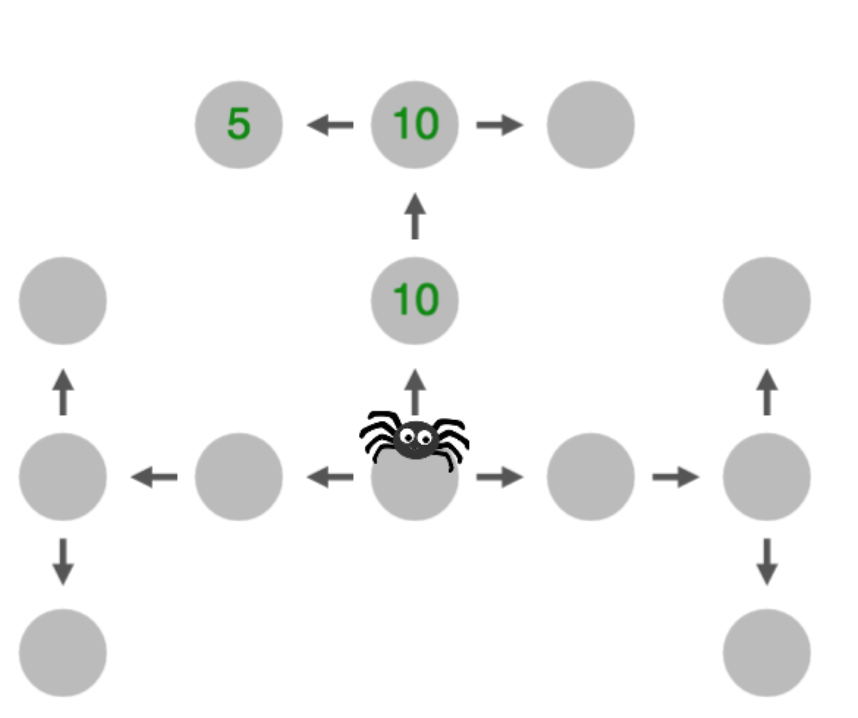
\includegraphics[width=0.4\textwidth]{figures/web-of-cash.png}
    \label{fig:MouselabMDP}
    \caption{Illustration of the Mouselab-MDP paradigm.}
\end{figure}
